%  This is a LaTex file.

%  Homework for the course "AMath 585:  Applied Linear Algebra and Numerical Analysis", 
%  Autumn quarter, 2009, Anne Greenbaum.


%   A latex format for making homework assignments.


\documentclass[letterpaper,12pt]{article}

%          The page format, somewhat wider and taller page than in art12.sty.

\topmargin -0.1in \headsep 0in \textheight 8.9in \footskip 0.6in
\oddsidemargin 0in  \evensidemargin 0in  \textwidth 6.5in
\usepackage{graphicx}
\usepackage{listings}
\usepackage{caption}
\usepackage{subcaption}
\usepackage{color}
\usepackage{float}
\definecolor{keywords}{RGB}{255,0,90}
\definecolor{comments}{RGB}{0,0,113}
\definecolor{red}{RGB}{160,0,0}
\definecolor{green}{RGB}{0,150,0}
\definecolor{codegreen}{rgb}{0,0.6,0}
\definecolor{codegray}{rgb}{0.5,0.5,0.5}
\definecolor{codepurple}{rgb}{0.58,0,0.82}
\definecolor{backcolour}{rgb}{0.95,0.95,0.92}
\definecolor{brown}{rgb}{0.59, 0.29, 0.0}
\definecolor{beaublue}{rgb}{0.74, 0.83, 0.9}
\definecolor{orange}{rgb}{1.0, 0.5, 0.0}
\definecolor{darkslategray}{rgb}{0.18, 0.31, 0.31}
\definecolor{deepblue}{rgb}{0,0,0.5}
\definecolor{deepred}{rgb}{0.6,0,0}
\definecolor{deepgreen}{rgb}{0,0.5,0}
\lstdefinestyle{myMatlabstyle}{
	language=Matlab,
	backgroundcolor=\color{white},   
	commentstyle=\color{codegreen},
	keywordstyle=\color{blue},
	%identifierstyle=\color{brown},
	numberstyle=\tiny\color{codegray},
	stringstyle=\color{orange},
	basicstyle=\footnotesize,
	breakatwhitespace=false,         
	breaklines=true,                 
	captionpos=b,                    
	keepspaces=true,                 
	numbers=left,                    
	numbersep=5pt,                  
	showspaces=false,                
	showstringspaces=false,
	showtabs=false,                  
	tabsize=2
}
\lstdefinestyle{myPythonstyle}{
	language=Python, 
	basicstyle=\ttfamily\small, 
	keywordstyle=\color{blue},
	backgroundcolor=\color{white}, 
	commentstyle=\color{green},
	stringstyle=\color{red},
	showstringspaces=false,
	%identifierstyle=\color{brown},
	breaklines=true, 
}
\lstset{language=Matlab,frame=single}
\lstset{language=Python,frame=single}
\usepackage{amsmath}
\usepackage{epsfig} 
% matrix environment
\newenvironment{mat}{\left[ \begin{array}{ccccccccccccc}}{\end{array}\right]}
\newcommand\bcm{\begin{mat}}
\newcommand\ecm{\end{mat}}

\begin{document}


%          Definitions of commonly used symbols.



%          The title and header.
\noindent
{\scriptsize AMath 585, Winter 2018} \hfill 

\begin{center}
\large
Assignment 7.
\normalsize

Jithin D. George, No. 1622555
\end{center}

\noindent
Due Friday, Feb. 16.
\vspace{.3in}

%           The questions!



\noindent

\begin{enumerate}
\item
The conjugate gradient method for solving a symmetric positive definite linear system
$Ax=b$ can be written as below:
\vspace{.1in}

\begin{center}
\begin{tabular}{|l|} \hline
Given $x_0$, compute $r_0 = b - A x_0$, and set $p_0 = r_0$. \\
For $k=1,2, \ldots$, \\
$~~$ Compute $A p_{k-1}$. \\
$~~$ Set $x_k = x_{k-1} + a_{k-1} p_{k-1}$, where $a_{k-1} = \frac{\langle r_{k-1} , r_{k-1} \rangle}
{\langle p_{k-1} , A p_{k-1} \rangle}$. \\
$~~$ Compute $r_k = r_{k-1} - a_{k-1} A p_{k-1}$. \\
$~~$ Set $p_k = r_k + b_{k-1} p_{k-1}$, where $b_{k-1} = \frac{\langle r_k , r_k \rangle}
{\langle r_{k-1} , r_{k-1} \rangle}$. \\
Endfor \\ \hline
\end{tabular}
\end{center}
\vspace{.1in}

\begin{enumerate}
\item
Show that the residual vectors $r_0 , \ldots , r_k$ are orthogonal to each other
($\langle r_i , r_j \rangle = 0$ if $i \neq j$) and that the direction vectors 
 $p_0 , \ldots , p_k$ are $A$-orthogonal ($\langle p_i , A p_j \rangle = 0$ if $i \neq j$).
[Hint:  First show that $\langle r_1 , r_0 \rangle = \langle p_1 , A p_0 \rangle = 0$
and then use induction on $k$.]

{\bf Solution:}

\[\langle r_1 , r_0 \rangle =  \langle r_0 - a_0 Ap_0 , r_0 \rangle =  \langle r_0 ,r_0 \rangle  - \frac{\langle r_{0} , r_{0} \rangle}
{\langle p_{0} , A p_{0} \rangle}\langle Ap_0 , r_0 \rangle \]
\[r_0 = p_0\]
\[\langle r_1 , r_0 \rangle = \langle r_0, r_0 \rangle  - \langle r_0, r_0 \rangle   = 0 \]

\[\langle p_1 , A p_0 \rangle = \langle r_1 + b_{0} p_{0} , A p_0 \rangle = \langle r_1 , A p_0 \rangle +  \langle b_{0} p_{0} , A p_0 \rangle  \]

\[= \langle r_1 , A p_0 \rangle +  \frac{1}{a_0}\langle r_1 , r_1 \rangle \]
\[= \langle r_1 , A p_0 \rangle +  \frac{1}{a_0}\langle r_1 , r_0 - a_0 Ap_0 \rangle \]
\[= \langle r_1 , A p_0 \rangle +  \frac{1}{a_0}\langle r_1 , r_0 \rangle - \langle r_1, Ap_0 \rangle \]
\[=0\]

Assume for j from 1 to k,
\[\langle r_j , r_{k+1} \rangle =0 , \langle p_{j} , A p_{k+1} \rangle = 0\]

\[\langle r_{k+2} , r_{k+1} \rangle =  \langle r_{k+1} - a_{k+1} Ap_{k+1} , r_{k+1} \rangle =  \langle r_{k+1} ,r_{k+1} \rangle  - \frac{\langle r_{k+1} , r_{k+1} \rangle}
{\langle p_{k+1} , A p_{k+1} \rangle}\langle Ap_{k+1} , r_{k+1} \rangle \]
\[\langle r_{k+2} , r_{k+1} \rangle =    \langle r_{k+1} ,r_{k+1} \rangle  - \frac{\langle r_{k+1} , r_{k+1} \rangle}
{\langle p_{k+1} , A p_{k+1} \rangle}\langle Ap_{k+1} , p_{k+1} \rangle +\frac{\langle r_{k+1} , r_{k+1} \rangle}
{\langle p_{k+1} , A p_{k+1} \rangle}\langle Ap_{k+1} , b_k p_{k} \rangle \] 
\[=    \langle r_{k+1} ,r_{k+1} \rangle  - \langle r_{k+1} , r_{k+1} \rangle+a_{k+1}b_k \langle Ap_{k+1} ,  p_{k} \rangle \]
\[=    0\]
For j from 1 to k,
\[\langle r_{k+2} , r_{j} \rangle =    \langle r_{k+1} ,r_{j} \rangle  - a_{k+1}
\langle Ap_{k+1} , p_{j} \rangle +a_{k+1}b_k\langle Ap_{k+1} , b_k p_{j-1} \rangle \] 
\[=    0+0+0 =    0\]

\[\langle p_{k+2} , A p_{k+1} \rangle = \langle r_{k+2} , A p_{k+1} \rangle+  b_{k+1}\langle p_{k+1} , A p_{k+1} \rangle \]
\[= \langle r_{k+2} , A p_{k+1} \rangle+  \frac{1}{a_{k+1}}\langle r_{k+2} , r_{k+2} \rangle \]
\[= \frac{1}{a_{k+1}} \langle r_{k+2} , r_{k+1}- r_{k+2} \rangle+  \frac{1}{a_{k+1}}\langle r_{k+2} , r_{k+2} \rangle \]
\[= \frac{1}{a_{k+1}} \langle r_{k+2} , r_{k+1}\rangle- \frac{1}{a_{k+1}} \langle r_{k+2} , r_{k+2} \rangle+  \frac{1}{a_{k+1}}\langle r_{k+2} , r_{k+2} \rangle \]
\[=0\]
For j from 1 to k,
\[\langle p_{k+2} , A p_{j} \rangle = \langle r_{k+2} , A p_{j} \rangle+  b_{k+1}\langle p_{k+1} , A p_{j} \rangle \]
\[= \langle r_{k+2} , A p_{j} \rangle+  0 \]
\[= \frac{1}{a_{j}} \langle r_{k+2} , r_{j}- r_{j+1} \rangle\]
\[= \frac{1}{a_{k+1}} \langle r_{k+2} , r_{j}\rangle- \frac{1}{a_{j}} \langle r_{k+2} , r_{j+1} \rangle\]
\[=0+0 =0\]
Since the induction step works, it is thus proved that all k+1 residual vectors are orthogonal.
\item
If $A$ is the $N \times N$ matrix of the 5-point operator for Poisson's equation on a square,
count the number of operations (additions, subtractions, multiplications, and divisions) performed
in each iteration.  (Show how you arrive at your result.)

{\bf Solution:}



Multiplying one row of A with a vector is 5 multiplications and 4 additions. Thus, $Ap$ takes 9 N operations. Similarly, an inner product takes $2N-1 \approx 2N $ operations. Vector additions and scalar vector multiplication take N operations. $a_{k-1}$ takes 4N but $b_{k-1}$ takes 2N because one inner product has been done before. 

\begin{center}
\begin{tabular}{|l|} \hline

$\textcolor{red}{9N~~~~~~~~~~~~~~~~~~~~~}$ Compute $A p_{k-1}$. \\
$\textcolor{red}{6N=N+N+4N}$ Set $x_k = x_{k-1} + a_{k-1} p_{k-1}$, where $a_{k-1} = \frac{\langle r_{k-1} , r_{k-1} \rangle}
{\langle p_{k-1} , A p_{k-1} \rangle}$. \\
$\textcolor{red}{2N~~~~~~~~~~~~~~~~~~~~}$ Compute $r_k = r_{k-1} - a_{k-1} A p_{k-1}$. \\
$\textcolor{red}{4N =N+N+2N}$ Set $p_k = r_k + b_{k-1} p_{k-1}$, where $b_{k-1} = \frac{\langle r_k , r_k \rangle}
{\langle r_{k-1} , r_{k-1} \rangle}$. \\ \hline
\end{tabular}
\end{center}
\vspace{.1in}

Thus, CG has a total of 21 N operations.

\item
Compare your operation count in (b) to that of a Gauss-Seidel iteration applied to the
same $N$ by $N$ 5-point matrix $A$.  Also compare to the operation count for a multigrid 
V-cycle, using one Gauss-Seidel iteration on each visit to each grid level.
(Again, show how you derive your operation counts.)
\end{enumerate}


{\bf Solution:}



\textcolor{blue}{Gauss Seidel iteration:}
\[u^{k+1} = M^{-1}Nu_k + M^{-1}f\]
M is lower triangular with diagonal terms. To find its inverse, we have to solve these equations, which I do with back substitution.
\[ \bcm a &0 &0 &0\\ b &c &0&0\\d &e &f&0\\g &h &i&j\\\ecm \bcm u_1\\u_2\\u_3\\u_4\ecm = \bcm f_1\\f_2\\f_3\\f_4\ecm \]
The first line would take 1 operation(division). The second line would take 3(2 divisions and 1 subtraction). The third line would be 5 operations. The fourth 7. The Nth would take 2N-1. So, totally, it would take $N^2$ operations (the sum of the first N odd numbers).

However if you have the lower triangular part of the Poisson matrix, the number of operations would in each line would 1,3,5,5,5,5,.... Thus, total number of operations needed would be 5N.
 
N has two elements on each row. So, $Nu_k$ would be 3N operations. (2 multiplications and 1 addition on every line) 
 
 Thus, total number of operations needed for Gauss-Seidel would be 13 N ($M^{-1}Nu_k = 5N +3N= 8 N$ and $M^{-1}F = 5N$).
 
\textcolor{blue}{V-cycle:} 
\begin{itemize}
\item 
Going Down:

Gauss Seidel : 
\[13N + 13\frac{N}{4}+13\frac{N}{16}+ \ldots \approx  13\frac{4}{3}N = 17.33N\]


Projection :
Projection involves one multiplication in each row. So, N operations
\[N + \frac{N}{4}+\frac{N}{16}+ \ldots \approx  \frac{4}{3}N \]
\item
Bottom Level :

Operations : c (Constant)

\item Going Up:
Gauss Seidel : 
\[13N + 13\frac{N}{4}+13\frac{N}{16}+ \ldots \approx  13\frac{4}{3}N = 17.33N\]
Interpolation :
Projection involves two multiplications in each row. So, N operations
\[2N + \frac{2N}{4}+\frac{2N}{16}+ \ldots \approx  \frac{8}{3}N \] 
\item
Final Step
\[x_k = x_{k-1}+e\]
N operations.
\end{itemize}


Total number of operations for a V-cycle = 38.66 N +c
 .


\item
Implement a 2-grid method for solving the 1D model problem with homogeneous Dirichlet
boundary conditions:
\[
u_{xx} = f(x) ,~~u(0) = u(1) = 0.
\]
Use linear interpolation to go from the coarse grid with spacing $2h$ to the fine grid
with spacing $h$.  Take the projection matrix $I_h^{2h}$, going from the fine grid to the
coarse grid, to be $0.5$ times the transpose of the interpolation matrix: 
$I_h^{2h} = \frac{1}{2} ( I_{2h}^h )^T$.
Use a multigrid V-cycle with 1 smoothing step on each visit to each grid level. 
Try weighted Jacobi and Gauss-Seidel as the smoothing step.
Try several different values of the mesh spacing $h$ and show that you achieve convergence to
a fixed tolerance in a number of cycles that is independent of the mesh size.

{\bf Solution:}



\begin{figure}[H]
    \centering
    \begin{subfigure}[b]{0.45\textwidth}
        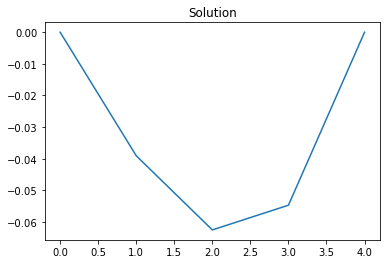
\includegraphics[width=\textwidth]{solution}
        \caption{Solution}
        \label{fig:gull}
    \end{subfigure}
    ~ %add desired spacing between images, e. g. ~, \quad, \qquad, \hfill etc. 
      %(or a blank line to force the subfigure onto a new line)
    \begin{subfigure}[b]{0.45\textwidth}
        \includegraphics[width=\textwidth]{convergence}
        \caption{Iterations needed}
        \label{fig:tiger}
    \end{subfigure}
    ~ %add desired spacing between images, e. g. ~, \quad, \qquad, \hfill etc. 
    %(or a blank line to force the subfigure onto a new line)

    \caption{$u_{xx} = \sin(\pi x) $}\label{fig:animals}
\end{figure}

The number of cycles needed becomes independent of mesh size
\begin{lstlisting}[style=myPythonstyle]
import numpy as np
import scipy 
import matplotlib.pyplot as plt

def pmatrix(n):
    #n internal points to n/2
    L = np.zeros((int(n/2),n))
    for i in range(int(n/2)):
        p = int(2*(i+1)-1)
        L[i,p]=1
    return L
def imatrix(n):
    #n/2 to n internal points
    L = np.zeros((n,int(n/2)))
    L[0,0] = 0.5
    for i in range(1,int(n/2)):
        a = 2*i-1
        b = i-1
        L[a,b]=1
        L[a+1,b]=0.5
        L[a+1,b+1]=0.5
    L[-1,-1]=1
    return L
n = 10

def jacobi_step(u,A,f):
    p = np.diag(A)
    M  = np.diag(p)
    invM = np.diag(1/p)
    N = M - A
    G = np.dot(invM,N)
    c = np.dot(invM,f)
    return np.dot(G,u)+c

def GS_step(u,A,f):
    M  = np.tril(A)
    #invM = np.diag(1/p)
    N = M - A
    G = scipy.linalg.solve(M,N)
    c = scipy.linalg.solve(M,f)
    return np.dot(G,u)+c

def weighted_step(u,A,f,w=2/3):
    u_n = jacobi_step(u,A,f) 
    return (1-w)*u+w*u_n
def tridiag(a, b, c, k1=-1, k2=0, k3=1):
    return np.diag(a, k1) + np.diag(b, k2) + np.diag(c, k3)   
def multigrid(f,x_0,smoother):
    n = len(f)
    h = 1/(n+1)
    A = makeA(n)
    A_c = makeA(int(n/2))
    pmat = pmatrix(n)
    imat = imatrix(n)
    x = x_0
    for i in range(100):
        #print(len(x))
        x = smoother(x,A,f)
        r = f - np.dot(A,x)
        r_c = np.dot(pmat,r)
        e_c = np.linalg.solve(A_c,r_c)
        e = np.dot(imat,e_c)
        x = x+e
        if np.linalg.norm(e, np.inf) < 0.001:
            #print(i)
            return x,i
    return x
n=70        
x_0 = 2*np.ones(n)
x1 = np.linspace(0,1,n+2)

f = np.sin(np.pi*x1[1:-1])

def makeA(N):
    a = np.ones(N)
    b = np.ones(N-1)
    A = ((N+1)**2)*tridiag(b,-2*a,b)
    return A
g = []    
for n in range(10,300,2):       
        x_0 = 2*np.ones(n)
        x1 = np.linspace(0,1,n+2)        
        f = np.sin(np.pi*x1[1:-1])
        g+= [multigrid(f,x_0,GS_step)[1]]
        
s = []    
for n in range(10,300,2):       
        x_0 = 2*np.ones(n)
        x1 = np.linspace(0,1,n+2)        
        f = np.sin(np.pi*x1[1:-1])
        s+= [multigrid(f,x_0,weighted_step)[1]]

    
x = np.linspace(10,300,145)  
plt.plot(x,g,label = 'Gauss Seidel') 
plt.plot(x,s,label = 'Weighted Jacobi')
plt.legend() 
\end{lstlisting} 
\item
\begin{enumerate}
\item
Consider an iteration of the form 
\[
x_k = x_{k-1} + M^{-1} ( b - A x_{k-1} ) ,
\]
for solving a nonsingular linear system $Ax=b$.  Note that the error $e_k := A^{-1} b - x_k$
satisfies
\[
e_k = (I - M^{-1} A) e_{k-1} = \ldots = (I - M^{-1} A)^k e_0.
\]
Assume that $\| e_0 \|_2 = 1$ and that $\| I - M^{-1} A \|_2 = \frac{1}{2}$.
Estimate the number of iterations required to reduce the 2-norm of the error below $2^{-20}$.
Show how you obtain your estimate.  Now suppose you know only that the spectral radius
$\rho ( I - M^{-1} A ) = \frac{1}{2}$.  Can you give an estimate of the number of iterations
required to reduce the 2-norm of the error below $2^{-20}$?  Explain why or why not.


{\bf Solution:}


If we know $\| I - M^{-1} A \|_2 = \frac{1}{2}$,
\[
||e_k||_2 \leq \| I - M^{-1} A \|_2^k ||e_0||_2 \leq 2^{-k} .\]
To get the error below $2^{-20}$, we need 20 iterations.

If $I - M^{-1} A$ is normal, then $\rho ( I - M^{-1} A ) =\| I - M^{-1} A \|_2 $. So, we would only need 20.

If $I - M^{-1} A$ is diagonalizable with condition number $\kappa$

\[
||e_k||_2 \leq \| I - M^{-1} A \|_2^k ||e_0||_2 \leq \kappa^{k}   \]
\[\kappa^{k} =  2^{-20}  \]
\[k \log(\kappa) =  -20 \log(2)  \]
\[k = \frac{-20 \log(2) }{\log(\kappa)}   \]

Without the condition number, we cannot determine the bounds.

\item
Consider the GMRES algorithm applied to an $n$ by $n$ matrix $A$ with the sparsity pattern 
pictured below:
\[
\left[ \begin{array}{ccccc}
\ast & \ast & \cdots & \ast & \ast \\
\ast & \ast & \cdots & \ast & 0 \\
0    & \ast & \cdots & \ast & 0 \\
\vdots  & \ddots & \ddots & \vdots & \vdots \\
0    & \cdots    & \cdots & \ast & 0 \end{array} \right] ,
\]
where the $\ast$'s represent nonzero entries.  Show that if the initial residual is the 
$n$th unit vector $( 0, \ldots , 0 , 1 )^T$, then the algorithm makes no progress
until step $n$.  Show that a matrix with this sparsity pattern can have {\em any}
eigenvalues.  Conclude that eigenvalue information alone cannot be enough to ensure
fast convergence of the GMRES algorithm.


{\bf Solution:}

\[Ar_0 =  \bcm *\\  0\\ 0\\ \vdots \\ 0 \ecm, A^2r_0 =  \bcm *\\  *\\ 0\\\vdots \\ 0 \ecm\]
For k = 1: n - 1
\[\langle r_0, A^k r_0 \rangle = 0\]
\[r_k = r_0 - AQy\]
The columns of Q span [$r_0, Ar_0, A^2r_0, \ldots $].

The columns of AQ span [$Ar_0, A^2r_0, A^3r_0, \ldots $].

\[r_k = r_0 - \sum_{i=1}^{k} y_i  AQ\]
\[r_k = r_0 - \sum_{i=1}^{k} y_i c_i A^ir_0\]
We choose the y that minimizes $||r_k||_2$. For k from 1 to n-1, since $r_0$ is orthogonal to $A^ir_0$, the y vector is simply zero.
Thus, for k from 1 to n-1,
\[r_k = r_0\]

The matrix
\[ \bcm a &b &c \\ 1 &0 &0\\0 &1 &0\ecm\]
 has the following characteristic polynomial.
\[-a\lambda^2-b\lambda-c+\lambda^3\]
The matrix
\[ \bcm a &b &c &d\\ 1 &0 &0&0\\0 &1 &0&0\\0 &0 &1&0\\\ecm\]
 has the following characteristic polynomial.
 \[-a\lambda^3-b\lambda^2-c\lambda-d+\lambda^4\]
This patterns extends to bigger and bigger matrices. So, we can assume that it is general. This matrix follows the same sparsity layout as the matrix in the question. Thus, our matrix has the same characteristic polynomial. Since the coefficients of the polynomial can be any number, the eigenvalues can be any number.

\end{enumerate}
\end{enumerate}

\end{document}

